
\chapter{The What and Wherefore of Topic Models}
\label{ch:intro}

Imagine that you are an intrepid reporter with an amazing scoop: you have
twenty-four hours of exclusive access three decades of e-mails sent within a
corrupt corporation.  You know there's dirt and scandal there, but it has been
well-concealed by the corporation's political friends.  How are you going to
understand this haystack well enough to explain it to your devoted readers under
such a tight deadline?

\section{Tell me about your haystack}

Unlike the vignette above, interacting with large text data sets is often posed
as a needle in a haystack problem.  The poor user---faced with documents that
would take a decade to read---is looking for a single needle: a document (or at
most a handful of documents) that matches what the user is looking for.  This
could be a ``smoking gun'' e-mail, the document that best represents a
concept~\citep{Salton-68} or the answer to a question~\citep{Hirschman-01}.

These questions are important.  The sub-discipline of information retrieval is
built upon systematizing, solving, and evaluating this problem.  Google's empire
is built on the premise of users typing a few keywords into a search engine box
and seeing quick, consistent search results.  However, this is not the only
problem that confronts those interacting with large text datasets.

A different, but related problem is \emph{understanding} large document
collections, common in science policy~\citep{talley-11}, journalism, and the
humanities~\citep{moretti-13}.  There is not just one precious needle in
the haystack.  At the risk of abusing the metaphor, \emph{sometimes you care
  about the straw}.  Instead of looking for a smoking gun alerting to you some
crime that was committed, perhaps you are looking for a sin of
omission: did this company never talk about diversity in its workforce?
Instead of a single answer to a question, perhaps you are looking for a diversity
of responses: what are the different ways that people account for rising income
inequality?  Instead of looking for one document, perhaps you want to provide
population level statistics: what proportion of Twitter users have ever talked
about gun violence?

At first, it might seem that answering these questions would require building an
extensive ontology or categorization scheme.  For every new corpus, you would need to define  the buckets that a document could fit into, politely ask some librarians and
archivists to put each document into the correct buckets, perhaps automate the
process with some supervised machine learning, and then collect summary
statistics when you are done.

Obviously, such laborious processes are possible---they have been done
for labeling congressional
speeches\footnote{\url{www.congressionalbills.org/}} and understanding
emotional state~\cite{wiebestates}---and remain an important part of
social science, information science, library science, and machine
learning.  But these processes are not always possible, fast, or even
the optimal outcome if we had infinite resources.  First, they
 require a significant investment of time and resources.
Even creating the \emph{list} of categories is a difficult task and
requires careful deliberation and calibration.  Even if it were possible, a
particular question might not warrant the time or effort: the \oe{}vre
of a minor author (only of interest to a few), or the tweets of a day
(not relevant tomorrow).

This survey explores the ways that humans and
computers make sense of document collections through tools called topic models.
Topic models allow us to answer big-picture questions quickly, cheaply, and without human intervention.
Once trained, they provide a framework for humans to understand document collections both directly by ``reading'' models or indirectly by using topics as input variables for further analysis.
For readers already comfortable with topic models, feel free to skip this
chapter; we will mostly cover the definitions and implementations of topic models.

The intended audience of this book is a reader with some knowledge of
document processing (e.g., knows what ``tokens'' and ``documents''
are), basic understanding of some probability (e.g., what a
distribution is), and interested in many application domains.  For
each of the application areas we discuss, we attempt to introduce and
motivate each domain to an outsider.  By the
end of the book (Chapter~\ref{ch:building}), we hope that the reader
will be excited enough to attempt to embark on building their own
topic models.  In this chapter, we go deeper into more of the
implementation details.  Readers who are already topic model experts
will likely not learn much technically, but we hope our coverage of
diverse applications will expose a topic modeling expert to models and
approaches they had not seen before.

\section{What is a Topic Model}

Returning to our motivating example, consider the e-mails from Enron, the prototypical
evil corporation of the turn of the century.  Imagine that you're an
investigative reporter, the first to get your hands on Enron e-mails.  You know
that wrongdoing happened, but you do not know who did it or how it was planned
and carried out.  You have suspicions (e.g., around the California energy spot market),
but you are curious to know if there are other skeletons in the closet, and
you're highly motivated to find them.

So you run a topic model on the data.  True to its name, a topic model
gives you ``topics'', collections of words that make sense together.
Looking at the Enron e-mails, we can see topics about gas contracts,
California regulators, and stock prices
(Figure~\ref{fig:enron_topics}).

\begin{figure}
\begin{center}
  \begin{tabular}{ccccc}
    Topic 3    & Topic 6   & Topic 9    & Topic 14 & Topic 22 \\
    \hline
    trading    & gas       & state      & ferc     & group \\
    financial  & capacity  & california & issue    & meeting \\
    trade      & deal      & davis      & order    & team \\
    product    & pipeline  & power      & party    & process \\
    price      & contract  & utilities  & case     & plan \\
    \hline
  \end{tabular}
\end{center}

  \caption{Five topics from a twenty-five topic model fit on Enron
    e-mails.  Example topics concern financial transactions, natural
    gas, the California utilities, federal regulation, and planning
    meetings.  We provide the five most probable words from each topic
  (each topic is a distribution over all words).}
  \label{fig:enron_topics}
\end{figure}

The first half of a topic model connects topics to a jumbled ``bag of words''.
When we say that a topic is about $X$, we are manually assigning a \textit{post hoc} label
 (more on this in Chapter~\ref{sec:display}).
It remains the responsibility of the human consumer of topic models to go further and
make sense of these piles of straw (we discuss labeling the topics
more in Chapter~\ref{ch:viz}).

\begin{figure}

\begin{center}
\colorbox{gray}{ \parbox{.9\linewidth}{
Yesterday, SDG\&E filed a motion for adoption of an
electric procurement cost recovery mechanism and for an order
shortening time for parties to file comments on the mechanism. The
attached email from SDG\&E contains the motion, an executive summary,
and a detailed summary of their proposals and recommendations
governing procurement of the net short energy requirements for
SDG\&E's customers. The utility requests a 15-day comment period, which
means comments would have to be filed by September 10 (September 8
is a Saturday). Reply comments would be filed 10 days later.}}

\begin{tabular}{ccl}
  Topic & Probability \\
  \hline
  9 & 0.42  \\
  11 & 0.05 \\
  8 & 0.05 \\
  \hline
\end{tabular}
\end{center}
  \caption{Example document from the Enron corpus and its association
    to topics.  Although it doesn't contain the word ``California'',
    it discusses a single California utility's dissatisfaction with how
    much it is paying for electricity.}
  \label{fig:enron_doc}
\end{figure}

Making sense of one of these word piles by itself can be difficult.
The second half of a topic model links topics to individual documents.
For example, the document in
Figure~\ref{fig:enron_doc} is about a California utility's reaction to
the short-term electricity market and exemplifies Topic~9 from
Figure~\ref{fig:enron_topics}.
Considering examples of documents that are strongly connected to a topic, along with the words associated with the topic, can give us a more complete representation of the topic.
If we get a sense that Topic~9 is of
interest, we can explore deeper to find other documents.

\section{Foundations}

\begin{center}
\begin{figure}
  \begin{center}
  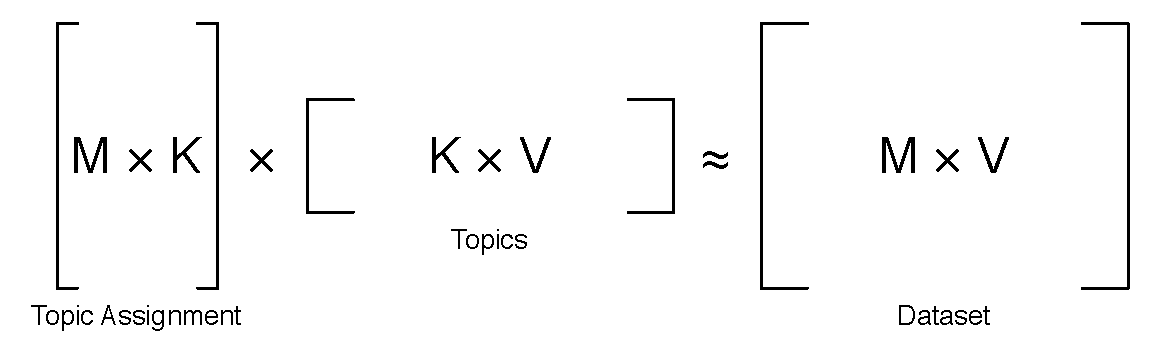
\includegraphics[width=.8\linewidth]{figures/matrix_factorization}
  \end{center}

  \caption{A matrix formulation of finding $K$ topics for a dataset
    with $M$ documents and $V$ unique words.  While this
    view of topic modeling includes approaches such as latent semantic
    analysis (\abr{lsa}), we focus on probabilistic techniques in the
    rest of this survey.}
  \label{fig:matrix_topics}
\end{figure}
\end{center}

You might notice that we are using the general term ``topic model''.
There are many specific mathematical formulations of topic models, and many algorithms that learn the parameters of those models from data.
Although we will focus on particular models and algorithms, we choose our terminology in order to emphasize that the similarities between formulations, models, and algorithms are often greater than their differences.

Topic modeling began with a linear algebra approach~\citep{deerwester-90} called
latent semantic analysis (\abr{lsa}): find the best low rank approximation of a
document-term matrix (Figure~\ref{fig:matrix_topics}).  While these approaches
have seen a resurgence in recent years~\citep{anandkumar-12:lda,arora-13}, we
focus on probabilistic approaches \cite{hofmann-99,papadimitriou-00,blei-03}, which are intuitive, work well, and allow for
easy modification (as we see later in many of our later chapters).

\begin{figure}
\small
  \begin{tabular}{cccc}
    Distribution & Density & Example Parameters & Example draws \\
    \hline
    Gaussian  & $\frac{1}{\sqrt{2 \sigma^2 \pi}} e^{- \frac{(x-\mu)^2}{2 \sigma^2}}$ & $\mu=2, \sigma^2=1.1$ & $x=2.21$\\
    Discrete  & $\prod_i \phi_i^{\ind{w=i}}$ & $\phi=(0.1, 0.6, 0.3)$
                                                & $w=2$ (second
                                                  item) \\
   Dirichlet & $\frac{\prod_{i=1}^K \Gamma(\alpha_i)}{\Gamma \left( \sum_{i=1}^K \alpha_i \right)} \prod_{i=1}^K \theta_i^{\alpha_i - 1} $ & $\alpha = (1.1, 0.1, 0.1)$  & $\theta = (0.8, 0.15, 0.05)$ \\
     \hline
  \end{tabular}
  \caption{Examples of probability distributions used in the
    generative stories of topic models.}
  \label{fig:distribution_examples}
\end{figure}

Despite the similarity in terms, the meaning of ``topic'' in topic modeling is distinct from the meaning in many information retrieval settings.
There is a substantial and well-developed field of topic detection and tracking \cite{allan-02}.
In TDT, a topic is usually closer to an event or an individual story.
In contrast, topic models tend to identify more abstract latent factors.
For example, a TDT topic might include an earthquake in Haiti, whereas a topic model might represent the same event as a combination of topics such as Haiti, natural disasters, and international aid.

There has been some work on using topic models to detect emerging events by searching for changes in topic probability \cite{alsumait-08}.
But these methods tend to identify mainly the fact that an event has occurred, without necessarily identifying the specific features of that event.
Other work has found that more lexically specific methods than topic models are best for identifying memes and viral phrases \cite{leskovec-09}.

\subsection{Probabilistic Building Blocks}
\label{sec:intro_building_blocks}

In probabilistic models we want to find values for unobserved model variables that do a good job of explaining the observed data.
The first step in inference is to turn this process around, and assert a way to generate data given model variables.
Probabilistic models thus begin with a generative story: a recipe listing a sequence of random events
that creates the dataset we are trying to explain.
Figure~\ref{fig:distribution_examples} lists some of the key players in these
stories, how they are parameterized and what samples drawn from these distributions look like.  We will
briefly discuss them, as we will use them to build a wide variety of topic models
later.

\paragraph{Gaussian} If you know any probability distribution already,
it is (probably) the
Gaussian.  This distribution does not have a role in the most basic topic models that we will
discuss here, but it will later (e.g., Chapter~\ref{ch:css}).  We
include it because it is a useful point of comparison against the other
distributions we {\em are} using (since it is perhaps the easiest to understand and best
known). A Gaussian is a distribution over all real numbers (e.g., $0.0, 0.5,
-4.2, \pi$, \dots).  You can ask it to spit out a number, and it will give you
some real number between negative infinity and positive infinity.  But not all
numbers have equal probability.  Gaussian distributions are parameterized by a
mean $\mu$ and variance $\sigma^2$.  Most samples from the distribution will be
near the mean $\mu$; how close is determined by the variance: higher variances
will cause the samples to be more spread out.

\paragraph{Discrete}

While Gaussian distributions are over a continuous space, documents are
combinations of discrete symbols, usually word tokens.\footnote{An emerging trend in natural language
  processing research is to view words as embedded in a continuous space. We
  discuss these ``representation learning'' approaches and their connection to
  topic modeling in Chapter~\ref{ch:conc}, but even then models are still defined over a discrete set of words.}   Thus, we need a distribution
over discrete sets.

A useful metaphor for thinking about discrete distributions is a weighted die.
The number of faces on the die is its dimension, and each face is associated with a distinct
outcome.  Each face has its own probability of how likely that outcome is;
these probabilities are the parameters of a discrete distribution
(Figure~\ref{fig:distribution_examples}).

Topic models are described by discrete distributions (sometimes called
multinomial distributions) that describe the connection between words and topics (the first half) and topics and documents (the second half).  A distribution
over words is called a topic distribution; each of the topics gives
higher weights to some words more than others (e.g., in Topic 9 from
the Enron corpus, ``state'' and ``california'' have higher probability
than other words).  Each document also has an ``allocation'' for each
topic: documents are about a small handful of topics, and most
documents have very low weights for most of the possible topics.

\paragraph{Dirichlet}

Although discrete distributions are the star players in topic models, they are
not the end of the story.  We often begin with Dirichlet distributions.
Just as Gaussians produce real numbers and discrete distributions produce symbols from a finite set, Dirichlet distributions produce probability vectors that can be used as the parameters of discrete distributions.
Like the Gaussian distribution, they have parameters analogous to a mean and
variance.  The mean is called the ``base measure'' $\tau$ and is the expected
value of the Dirichlet distribution: the values you would get if you averaged many draws from the
Dirichlet.  The concentration parameter $\alpha_0$ controls how far away individual draws are from the base measure.
Note that we often combine these parameters into a single value for each dimension: $\alpha_k = \alpha_0 \tau_k$.

\begin{center}
\begin{figure}
  \centering
  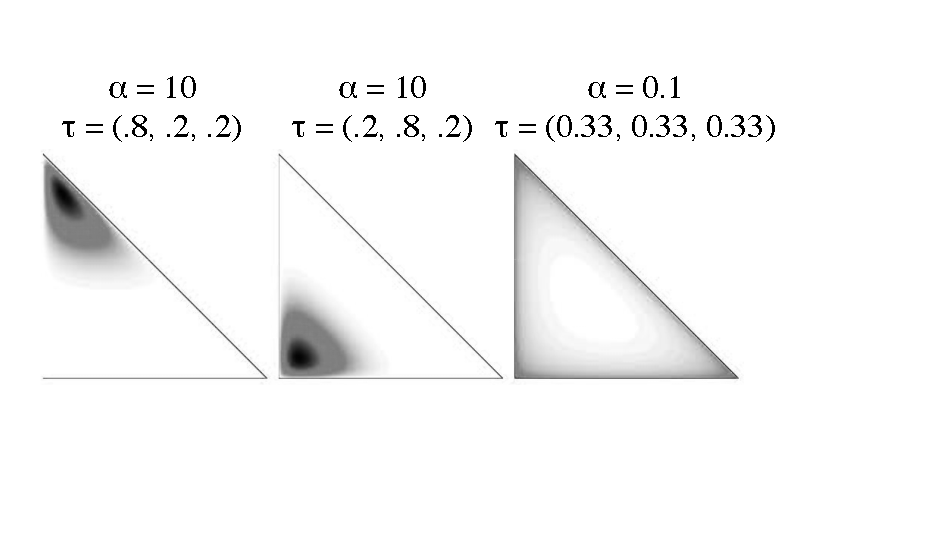
\includegraphics[width=.8\linewidth]{figures/dirichlet}
  \caption{Given different Dirichlet parameters, the Dirichlet
    distribution can either be informative (left, middle) or sparse
    (right).  Sparse distributions encourage distributions to favor
    only a small number of elements but do not care which ones.  This
    is consistent with our intuitions of how documents are written:
    they are only about a few things, and topics contain only a
    handful of words.}
  \label{fig:dirichlet_sparsity}
\end{figure}
\end{center}


If $\alpha_0$ is very large, then the draws from a Dirichlet will be very close to
$\tau$ (Figure~\ref{fig:dirichlet_sparsity}, left).  If $\alpha_0$ is small, however,
something more interesting happens: the discrete distributions become sparse
(Figure~\ref{fig:dirichlet_sparsity}, right).  A sparse distribution is a
distribution where only a few values have high probability and all other values are small.

Because topic models are meant to reflect the properties of real documents, modeling sparsity is important.  When a person sits down to write a document, they only
write about a handful of the topics that they could potentially use.  They do not write about every possible topic, and the sparsity of Dirichlet distributions is the probabilistic
tool that encodes this intuition.

There are several important special cases of the Dirichlet distribution.
If the base measure $\tau$ is uniform, we call the resulting distribution {\em symmetric}.
This case is appropriate when we do not expect any one element to be, on average, more likely than any other element across all samples from the distribution.
In the symmetric case the  distribution has only one parameter, the concentration $\alpha_0$.
If the base measure is uniform and the concentration parameter $\alpha_0$ is equal to the number of dimensions $K$ (or, equivalently, $\alpha_k = 1.0$ for all $k$), the distribution is uniform, placing equal probability on all $K$-dimensional probability distributions.


\section{Latent Dirichlet Allocation}
\label{sec:lda}

We now have all the tools we need to tell the complete story of the most popular topic model: latent Dirichlet allocation~\citep{blei-03}.  Latent
Dirichlet allocation\footnote{The name \abr{lda} is a play on \abr{lsa}, its
  non-probabilistic forerunner (latent semantic analysis).  Latent because we
  use probabilistic inference to infer missing probabilistic pieces of the
  generative story.  Dirichlet because of the Dirichlet parameters encoding
  sparsity.  Allocation because the Dirichlet distribution encodes the prior for
  each document's allocation over topics.} posits a ``generative process'' about
how the data came to be.  We assemble the probabilistic pieces to tell
this story about generating topics and how those topics are used to create
diverse documents.
We note that LDA is closely related to its probabilistic precursor, pLSA \cite{hofmann-99}, which can be viewed as a special case of LDA in which the Dirichlet priors are uniform.

\paragraph{Generating Topics}

The first part of the story is to create the topics.  The user specifies that
there are $K$ distinct topics.  Each of the $K$ topics is drawn from a Dirichlet
distribution with a uniform base distribution and concentration parameter
$\lambda$: $\phi_k \sim \dir{\lambda {\bm u}}$.  The discrete distribution
$\phi_k$ has a weight for \emph{every} word in the vocabulary.

However, when we summarize topics (as in
Figure~\ref{fig:enron_topics}), we typically only use the top (most probable) words of
a topic.  The lower probability words are less relevant to the topic
and thus are not shown.

\paragraph{Document Allocations}

Document allocations are distributions over topics for each document.  This
encodes what a document is about; the sparsity of the Dirichlet distribution's
concentration parameter $\alpha_0$ ensures that the document will only be about a
few topics.  Each document has a discrete distribution over topic: $\theta_d \sim
\dir{\alpha {\bm u}}$.

\paragraph{Words in Context}

Now that we know what each document is about, we need to actually create the
words that appear in the document.  We assume\footnote{It is possible to model
  this in the generative story as well, e.g., with a Poisson distribution.
  However, we often do not care about document \emph{lengths}---only what the
  document is about---so we can usually ignore this part of the story.} that
there are $N_d$ words in document $d$.  For each word $n$ in the
document $d$, we first choose a {\bf topic assignment} $z_{d,n} \sim
\disc{\theta_d}$.  This is one of the $K$ topics that tells us which topic the
word token is from, but not what the word is.

To select which word we will see in the document, we draw from the a discrete
distribution again.  Given a word token's topic assignment $z_{d,n}$, we draw from that
topic to select the word: $w_{d,n} \sim \phi_{z_{d,n}}$.  The topic assignment
tells you what the word is about, and then this selects which distribution over
words we use to generate the word.  % (Figure~\ref{fig:generative-ex}).

For example, consider the document in Figure~\ref{fig:enron_doc}.  To
generate it, we choose a distribution over all of the topics.  This is
$\theta$.  For this document, the distribution favors Topic~9 about
California.  The value for this topic is higher than any other topic.  For
each word in the document, the generative process chooses a topic
assignment $z_n$.  For this document, any topic is theoretically possible, but we expect that most of those will be Topic~9.

Then, for each token in the document, we need to choose which word type will appear.  This
comes from Topic~9's distribution over words (multiple topics have
word distributions shown in Figure~\ref{fig:enron_topics}).  Each is a
discrete draw from the topic's word distribution, which makes words
like ``California'', ``state'', and ``Sacramento'' more likely.

It goes without saying that the generative story is a fiction~\citep{box-87}.
Nobody is sitting down with dice to decide what to type in on their keyboard.
We use this story because it is \emph{useful}.  This fanciful story about randomly
choosing a topic for each word can help us because if we assume this generative
process, we can work backwards to find the topics that explain how a document
collection was created: every word, every document, gets associated with these
underlying topics.

This simple model helps us order our document collection: by assuming this story, we
can discover \emph{topics} (which certainly do not exist) so we can understand
the common themes that people use to write documents.  As we will see in later
chapters, slight tweaks of this generative story allow us to uncover more
complicated structures: how authors prefer specific topics, how topics change
over time, or how topics can be used across languages.

\section{Inference}

Given a generative model and some data, the process of uncovering the hidden
 pieces of the probabilistic generative story is called \emph{inference}.  More
concretely, it is a recipe for generating algorithms to go from data to
\emph{topics that explain a dataset}.

There are many flavors of algorithms for posterior inference: message
passing~\citep{zeng-13}, variational inference~\citep{blei-03},
gradient descent~\citep{hoffman-10}, and Gibbs
sampling~\citep{griffiths-04}.  All of these algorithms have their
advocates and reasons you should use them.  In this survey, we focus
on Gibbs sampling, which is simple, intuitive, and---with some clever
tricks specific to topic models---fast~\citep{yao-09}.  (We discuss
variational inference in Chapter~\ref{ch:building}.)

We present the results of Gibbs sampling without derivation,
which---along with the history of its origin in statistical
physics---are well described elsewhere.\footnote{We recommend
  \citet{resnik-09} for additional information on derivation.} We use
a variety of Gibbs sampling called \emph{collapsed} Gibbs sampling,
which allows inference to side-step some of the pieces of the
generative story: instead of explicitly representing the parameters of
a discrete distribution, distinct from any observations drawn from
that distribution, we represent the distribution solely through those
observations.  We can then recreate the topic and document
distributions through simple formulas as they are needed.

\subsection{Random Variables}

\paragraph{Topic Assignments}

Since every individual token is assumed to be generated from a single topic,
we can consider the {\em topic assignment} of a token as a variable.  For example,
an instance of the word ``compilation'' might be in a business topic in one
document and in an arts topic in another document.  Because each token has its own
topic assignment, it is even possible that the
same word might be assigned to different topics in the same document.
To estimate \emph{global} properties of the topic model we use aggregate statistics derived from these token-level topic assignments.

\paragraph{Document Allocation} The document allocation is a distribution over
the topics for each document; in other words, it says how popular each topic is
in a document.  If we count up how often a document uses a topic, this gives us
an idea of the popularity.  Let's define $\dc{d}{i}$ as the number of times
document~$d$ uses topic~$i$.  Clearly, this is larger for more popular topics;
however, it is not a probability because it is larger than one.  We can make it a
probability by dividing by the number of words in a document
\begin{equation}
\frac{\dc{d}{i}}{\sum_k \dc{d}{k}},
\label{eq:theta_ml}
\end{equation}
but this is problematic because it can sometimes give us zero and ignores the
influence of the Dirichlet distribution; a better estimate is\footnote{To be
  technical, Equation~\ref{eq:theta_ml} is a maximum likelihood estimate and
  Equation~\ref{eq:theta_map} is the maximum \textit{a posteriori}, which
  incorporates the influence of both the prior and the data.}
\begin{equation}
\theta_{d,i} \approx \frac{\dc{d}{i} + \alpha_i}{\sum_k \dc{d}{k} + \alpha_k}.
\label{eq:theta_map}
\end{equation}
It is important that this is never zero because we do not want it to rule out the possibility
that a topic is used in a particular document.  This helps the sampler
explore more of the possible combinations.

\paragraph{Topics}

Each topic is a distribution over words.  To understand what a topic is about,
we look at the profile of all of the tokens that have been assigned to that
topic.  We estimate the probability of a word in a topic as
\begin{equation}
\phi_{i,v} \approx \frac{\tc{i}{v} + \beta_v}{\sum_w \tc{i}{w} + \beta_w},
\label{eq:phi_map}
\end{equation}
where $\beta$ is the Dirichlet parameter for the topic distribution.

\subsection{Algorithm}

The collapsed Gibbs sampling algorithm for learning a topic model is
only based on the topic assignments, but we will use our estimates for
the topics $\phi_k$ and the documents $\theta_d$ discussed above.  We
begin by setting topic assignments randomly: if we have $K$ topics,
each word has equal chance to be associated with any of the topics.
These topics will be quite bad, looking like noisy copies of the
overall corpus distribution. But we will improve them one word at a
time.

The algorithm proceeds by sweeping over all word tokens in turn over and over.
At each iteration we change the topic assignments for each word in a way the reflects the
underlying probabilistic model of the data.  On average, each pass over the data makes the
topics slightly better until the model reaches a steady state.  There is no easy way
to tell when such a steady state has been reached, but eventually the topics will ``converge'' to something reasonable and you can consider yourself done.

The equation for the probability of assigning a word to a particular topic
combines information about words and about documents\footnote{To be theoretically correct, it is important
not to include the count associated with the token you are currently sampling in
these counts, which becomes more clear if the probability is written as
$p(z_{d,n}=j\,|\,z_{d,1}\dots z_{d,n-1},z_{d,n+1}\dots z_{d,N_d}, w_{d,n})$ to
show the dependence on the topic assignments of \emph{all other} token but not
this token.}
\begin{align}
p(z_{d,n}=j \g \dots) = \theta_d
\phi_j = \left(\frac{\dc{d}{i} + \alpha_i}{\sum_k \dc{d}{k} + \alpha_k} \right) \left( \frac{\tc{i}{w_{d,n}} + \beta_v}{\sum_w \tc{i}{w} +
    \beta_w} \right).
\label{eq:sampling}
\end{align}
Computing this value for each topic will result in a probability distribution over the topic assignment for this word token, given all the other topic assignments.  The next step is to randomly choose one of those indices with
probability proportional to the vector value.  You now assign that word to the
topic, update $\dc{}{}$ and $\tc{}{}$, and move on to the next word and repeat.
The two terms provide two ``pressures'', for global and local coherence. Sparsity in the topic-word distributions encourages tokens of the same word type to be assigned to a small number of topics,  regardless of where they occur. Sparsity in the document-topic distributions encourages tokens in the same document to be assigned to a small number of topics, regardless of what type they are.
For example, knowing that a word is ``compilation'' narrows down the number of potential topics considerably, but leaves ambiguity: is it program compilation or a music compilation? Knowing that the word occurs in a document with many other words in the \emph{arts} topic resolves this ambiguity, leaving the \emph{arts} topic as the most probable assignment.

At the very end of the algorithm, we can use the estimates of each topic
(Equation~\ref{eq:phi_map}) to summarize the main themes of the corpus and the
estimates of each document's topic distribution (Equation~\ref{eq:theta_map}) to
start exploring the collection automatically (Chapter~\ref{ch:ir}) or with a
human in the loop (Chapter~\ref{ch:viz}).

The algorithm that we have sketched here is the foundation of many of the more
advanced models that we will discuss later in the survey.  While we won't describe
the algorithms in detail, we will occasionally make reference to this sketch to
highlight challenges or difficulties in implementing topic models.

\subsection{Implementations}

Hopefully the previous algorithm sketch has convinced you that implementing
topic models is not a Herculean task; most skilled programmers can complete a
reasonable implementation of topic models in less than a day.  However, we would
suggest not trying to implement basic \abr{lda} if you just want the
output of a topic model, as there are many solid
implementations that help users get to useful results more quickly, particularly
as topic models often require extensive preprocessing.

Mallet is fast and is a widely used implementation in Java~\citep{mallet}.  This
is where you should probably start, in our biased opinion.  It runs in Java, uses
highly-optimized Gibbs sampling implementations, and can work from a variety of
text inputs.  It is well documented, mature, and runs well on a multi-core
machine, allowing it to process up to millions of documents.  Variational
inference is the other major option~\citep{blei-03,vw}, but often requires a
little more effort for new users to get a first result.

% Smola, Amr
However, if your corpus is truly large, it may be worthwhile
considering techniques that can be parallelized over large computer
clusters.  These techniques can be based on variational
inference~\citep{Narayanamurthy-11,zhai-12} or on
sampling~\citep{newman-08}.

While these implementations allow you to run \emph{specific} topic models, other
frameworks allow you to specify arbitrary generative
models.  This allows for quick prototyping of topic models and integrating topic
models with other probabilistic frameworks like regression or collaborative
filtering.  Examples of these general frameworks include
Stan~\citep{stan-software:2014}, Infer.net, and Church.

If you cannot find the specific model that you want among these
existing software packages, the flexibility and simplicity of topic
models and inference makes it relatively simple to adapt topic models
to model specific phenomena (as we describe in following chapters).

\section{Rest of this Survey}


In each of the following chapters, we focus on an application of topic
models, gradually increasing the complexity of the underlying models.
The chapters do occasionally refer to each other, but a reader should
be able to read each of the chapters independently.

The next chapter returns to the distinction between high level
overviews and finding a needle in a haystack.  We show how a high
level overview can help users and algorithms find documents of
interest.  We show how a high level overview can help
algorithms (Chapter~\ref{ch:ir}) and users (Chapter~\ref{ch:viz}) find documents
of interest.

These tools help enable new applications of topic models: how
understanding newspapers (Chapter~\ref{ch:nonfiction}) reveals the
march of history, how the corpus of writers of fiction
(Chapter~\ref{ch:fiction}) illuminates societal norms, how the
writings of science reveal innovation (Chapter~\ref{ch:sci}), or
how politicians' speeches (Chapter~\ref{ch:css}) reveal schisms in
political organizations.
